\documentclass{article} % For LaTeX2e
% Official ICLR 2027 style files (unmodified copies; hashes in BUILD.md).
\usepackage{iclr2027_conference,times}
%%%%% NEW MATH DEFINITIONS %%%%%

\usepackage{amsmath,amsfonts,bm}

% Mark sections of captions for referring to divisions of figures
\newcommand{\figleft}{{\em (Left)}}
\newcommand{\figcenter}{{\em (Center)}}
\newcommand{\figright}{{\em (Right)}}
\newcommand{\figtop}{{\em (Top)}}
\newcommand{\figbottom}{{\em (Bottom)}}
\newcommand{\captiona}{{\em (a)}}
\newcommand{\captionb}{{\em (b)}}
\newcommand{\captionc}{{\em (c)}}
\newcommand{\captiond}{{\em (d)}}

% Highlight a newly defined term
\newcommand{\newterm}[1]{{\bf #1}}


% Figure reference, lower-case.
\def\figref#1{figure~\ref{#1}}
% Figure reference, capital. For start of sentence
\def\Figref#1{Figure~\ref{#1}}
\def\twofigref#1#2{figures \ref{#1} and \ref{#2}}
\def\quadfigref#1#2#3#4{figures \ref{#1}, \ref{#2}, \ref{#3} and \ref{#4}}
% Section reference, lower-case.
\def\secref#1{section~\ref{#1}}
% Section reference, capital.
\def\Secref#1{Section~\ref{#1}}
% Reference to two sections.
\def\twosecrefs#1#2{sections \ref{#1} and \ref{#2}}
% Reference to three sections.
\def\secrefs#1#2#3{sections \ref{#1}, \ref{#2} and \ref{#3}}
% Reference to an equation, lower-case.
\def\eqref#1{equation~\ref{#1}}
% Reference to an equation, upper case
\def\Eqref#1{Equation~\ref{#1}}
% A raw reference to an equation---avoid using if possible
\def\plaineqref#1{\ref{#1}}
% Reference to a chapter, lower-case.
\def\chapref#1{chapter~\ref{#1}}
% Reference to an equation, upper case.
\def\Chapref#1{Chapter~\ref{#1}}
% Reference to a range of chapters
\def\rangechapref#1#2{chapters\ref{#1}--\ref{#2}}
% Reference to an algorithm, lower-case.
\def\algref#1{algorithm~\ref{#1}}
% Reference to an algorithm, upper case.
\def\Algref#1{Algorithm~\ref{#1}}
\def\twoalgref#1#2{algorithms \ref{#1} and \ref{#2}}
\def\Twoalgref#1#2{Algorithms \ref{#1} and \ref{#2}}
% Reference to a part, lower case
\def\partref#1{part~\ref{#1}}
% Reference to a part, upper case
\def\Partref#1{Part~\ref{#1}}
\def\twopartref#1#2{parts \ref{#1} and \ref{#2}}

\def\ceil#1{\lceil #1 \rceil}
\def\floor#1{\lfloor #1 \rfloor}
\def\1{\bm{1}}
\newcommand{\train}{\mathcal{D}}
\newcommand{\valid}{\mathcal{D_{\mathrm{valid}}}}
\newcommand{\test}{\mathcal{D_{\mathrm{test}}}}

\def\eps{{\epsilon}}


% Random variables
\def\reta{{\textnormal{$\eta$}}}
\def\ra{{\textnormal{a}}}
\def\rb{{\textnormal{b}}}
\def\rc{{\textnormal{c}}}
\def\rd{{\textnormal{d}}}
\def\re{{\textnormal{e}}}
\def\rf{{\textnormal{f}}}
\def\rg{{\textnormal{g}}}
\def\rh{{\textnormal{h}}}
\def\ri{{\textnormal{i}}}
\def\rj{{\textnormal{j}}}
\def\rk{{\textnormal{k}}}
\def\rl{{\textnormal{l}}}
% rm is already a command, just don't name any random variables m
\def\rn{{\textnormal{n}}}
\def\ro{{\textnormal{o}}}
\def\rp{{\textnormal{p}}}
\def\rq{{\textnormal{q}}}
\def\rr{{\textnormal{r}}}
\def\rs{{\textnormal{s}}}
\def\rt{{\textnormal{t}}}
\def\ru{{\textnormal{u}}}
\def\rv{{\textnormal{v}}}
\def\rw{{\textnormal{w}}}
\def\rx{{\textnormal{x}}}
\def\ry{{\textnormal{y}}}
\def\rz{{\textnormal{z}}}

% Random vectors
\def\rvepsilon{{\mathbf{\epsilon}}}
\def\rvtheta{{\mathbf{\theta}}}
\def\rva{{\mathbf{a}}}
\def\rvb{{\mathbf{b}}}
\def\rvc{{\mathbf{c}}}
\def\rvd{{\mathbf{d}}}
\def\rve{{\mathbf{e}}}
\def\rvf{{\mathbf{f}}}
\def\rvg{{\mathbf{g}}}
\def\rvh{{\mathbf{h}}}
\def\rvu{{\mathbf{i}}}
\def\rvj{{\mathbf{j}}}
\def\rvk{{\mathbf{k}}}
\def\rvl{{\mathbf{l}}}
\def\rvm{{\mathbf{m}}}
\def\rvn{{\mathbf{n}}}
\def\rvo{{\mathbf{o}}}
\def\rvp{{\mathbf{p}}}
\def\rvq{{\mathbf{q}}}
\def\rvr{{\mathbf{r}}}
\def\rvs{{\mathbf{s}}}
\def\rvt{{\mathbf{t}}}
\def\rvu{{\mathbf{u}}}
\def\rvv{{\mathbf{v}}}
\def\rvw{{\mathbf{w}}}
\def\rvx{{\mathbf{x}}}
\def\rvy{{\mathbf{y}}}
\def\rvz{{\mathbf{z}}}

% Elements of random vectors
\def\erva{{\textnormal{a}}}
\def\ervb{{\textnormal{b}}}
\def\ervc{{\textnormal{c}}}
\def\ervd{{\textnormal{d}}}
\def\erve{{\textnormal{e}}}
\def\ervf{{\textnormal{f}}}
\def\ervg{{\textnormal{g}}}
\def\ervh{{\textnormal{h}}}
\def\ervi{{\textnormal{i}}}
\def\ervj{{\textnormal{j}}}
\def\ervk{{\textnormal{k}}}
\def\ervl{{\textnormal{l}}}
\def\ervm{{\textnormal{m}}}
\def\ervn{{\textnormal{n}}}
\def\ervo{{\textnormal{o}}}
\def\ervp{{\textnormal{p}}}
\def\ervq{{\textnormal{q}}}
\def\ervr{{\textnormal{r}}}
\def\ervs{{\textnormal{s}}}
\def\ervt{{\textnormal{t}}}
\def\ervu{{\textnormal{u}}}
\def\ervv{{\textnormal{v}}}
\def\ervw{{\textnormal{w}}}
\def\ervx{{\textnormal{x}}}
\def\ervy{{\textnormal{y}}}
\def\ervz{{\textnormal{z}}}

% Random matrices
\def\rmA{{\mathbf{A}}}
\def\rmB{{\mathbf{B}}}
\def\rmC{{\mathbf{C}}}
\def\rmD{{\mathbf{D}}}
\def\rmE{{\mathbf{E}}}
\def\rmF{{\mathbf{F}}}
\def\rmG{{\mathbf{G}}}
\def\rmH{{\mathbf{H}}}
\def\rmI{{\mathbf{I}}}
\def\rmJ{{\mathbf{J}}}
\def\rmK{{\mathbf{K}}}
\def\rmL{{\mathbf{L}}}
\def\rmM{{\mathbf{M}}}
\def\rmN{{\mathbf{N}}}
\def\rmO{{\mathbf{O}}}
\def\rmP{{\mathbf{P}}}
\def\rmQ{{\mathbf{Q}}}
\def\rmR{{\mathbf{R}}}
\def\rmS{{\mathbf{S}}}
\def\rmT{{\mathbf{T}}}
\def\rmU{{\mathbf{U}}}
\def\rmV{{\mathbf{V}}}
\def\rmW{{\mathbf{W}}}
\def\rmX{{\mathbf{X}}}
\def\rmY{{\mathbf{Y}}}
\def\rmZ{{\mathbf{Z}}}

% Elements of random matrices
\def\ermA{{\textnormal{A}}}
\def\ermB{{\textnormal{B}}}
\def\ermC{{\textnormal{C}}}
\def\ermD{{\textnormal{D}}}
\def\ermE{{\textnormal{E}}}
\def\ermF{{\textnormal{F}}}
\def\ermG{{\textnormal{G}}}
\def\ermH{{\textnormal{H}}}
\def\ermI{{\textnormal{I}}}
\def\ermJ{{\textnormal{J}}}
\def\ermK{{\textnormal{K}}}
\def\ermL{{\textnormal{L}}}
\def\ermM{{\textnormal{M}}}
\def\ermN{{\textnormal{N}}}
\def\ermO{{\textnormal{O}}}
\def\ermP{{\textnormal{P}}}
\def\ermQ{{\textnormal{Q}}}
\def\ermR{{\textnormal{R}}}
\def\ermS{{\textnormal{S}}}
\def\ermT{{\textnormal{T}}}
\def\ermU{{\textnormal{U}}}
\def\ermV{{\textnormal{V}}}
\def\ermW{{\textnormal{W}}}
\def\ermX{{\textnormal{X}}}
\def\ermY{{\textnormal{Y}}}
\def\ermZ{{\textnormal{Z}}}

% Vectors
\def\vzero{{\bm{0}}}
\def\vone{{\bm{1}}}
\def\vmu{{\bm{\mu}}}
\def\vtheta{{\bm{\theta}}}
\def\va{{\bm{a}}}
\def\vb{{\bm{b}}}
\def\vc{{\bm{c}}}
\def\vd{{\bm{d}}}
\def\ve{{\bm{e}}}
\def\vf{{\bm{f}}}
\def\vg{{\bm{g}}}
\def\vh{{\bm{h}}}
\def\vi{{\bm{i}}}
\def\vj{{\bm{j}}}
\def\vk{{\bm{k}}}
\def\vl{{\bm{l}}}
\def\vm{{\bm{m}}}
\def\vn{{\bm{n}}}
\def\vo{{\bm{o}}}
\def\vp{{\bm{p}}}
\def\vq{{\bm{q}}}
\def\vr{{\bm{r}}}
\def\vs{{\bm{s}}}
\def\vt{{\bm{t}}}
\def\vu{{\bm{u}}}
\def\vv{{\bm{v}}}
\def\vw{{\bm{w}}}
\def\vx{{\bm{x}}}
\def\vy{{\bm{y}}}
\def\vz{{\bm{z}}}

% Elements of vectors
\def\evalpha{{\alpha}}
\def\evbeta{{\beta}}
\def\evepsilon{{\epsilon}}
\def\evlambda{{\lambda}}
\def\evomega{{\omega}}
\def\evmu{{\mu}}
\def\evpsi{{\psi}}
\def\evsigma{{\sigma}}
\def\evtheta{{\theta}}
\def\eva{{a}}
\def\evb{{b}}
\def\evc{{c}}
\def\evd{{d}}
\def\eve{{e}}
\def\evf{{f}}
\def\evg{{g}}
\def\evh{{h}}
\def\evi{{i}}
\def\evj{{j}}
\def\evk{{k}}
\def\evl{{l}}
\def\evm{{m}}
\def\evn{{n}}
\def\evo{{o}}
\def\evp{{p}}
\def\evq{{q}}
\def\evr{{r}}
\def\evs{{s}}
\def\evt{{t}}
\def\evu{{u}}
\def\evv{{v}}
\def\evw{{w}}
\def\evx{{x}}
\def\evy{{y}}
\def\evz{{z}}

% Matrix
\def\mA{{\bm{A}}}
\def\mB{{\bm{B}}}
\def\mC{{\bm{C}}}
\def\mD{{\bm{D}}}
\def\mE{{\bm{E}}}
\def\mF{{\bm{F}}}
\def\mG{{\bm{G}}}
\def\mH{{\bm{H}}}
\def\mI{{\bm{I}}}
\def\mJ{{\bm{J}}}
\def\mK{{\bm{K}}}
\def\mL{{\bm{L}}}
\def\mM{{\bm{M}}}
\def\mN{{\bm{N}}}
\def\mO{{\bm{O}}}
\def\mP{{\bm{P}}}
\def\mQ{{\bm{Q}}}
\def\mR{{\bm{R}}}
\def\mS{{\bm{S}}}
\def\mT{{\bm{T}}}
\def\mU{{\bm{U}}}
\def\mV{{\bm{V}}}
\def\mW{{\bm{W}}}
\def\mX{{\bm{X}}}
\def\mY{{\bm{Y}}}
\def\mZ{{\bm{Z}}}
\def\mBeta{{\bm{\beta}}}
\def\mPhi{{\bm{\Phi}}}
\def\mLambda{{\bm{\Lambda}}}
\def\mSigma{{\bm{\Sigma}}}

% Tensor
\DeclareMathAlphabet{\mathsfit}{\encodingdefault}{\sfdefault}{m}{sl}
\SetMathAlphabet{\mathsfit}{bold}{\encodingdefault}{\sfdefault}{bx}{n}
\newcommand{\tens}[1]{\bm{\mathsfit{#1}}}
\def\tA{{\tens{A}}}
\def\tB{{\tens{B}}}
\def\tC{{\tens{C}}}
\def\tD{{\tens{D}}}
\def\tE{{\tens{E}}}
\def\tF{{\tens{F}}}
\def\tG{{\tens{G}}}
\def\tH{{\tens{H}}}
\def\tI{{\tens{I}}}
\def\tJ{{\tens{J}}}
\def\tK{{\tens{K}}}
\def\tL{{\tens{L}}}
\def\tM{{\tens{M}}}
\def\tN{{\tens{N}}}
\def\tO{{\tens{O}}}
\def\tP{{\tens{P}}}
\def\tQ{{\tens{Q}}}
\def\tR{{\tens{R}}}
\def\tS{{\tens{S}}}
\def\tT{{\tens{T}}}
\def\tU{{\tens{U}}}
\def\tV{{\tens{V}}}
\def\tW{{\tens{W}}}
\def\tX{{\tens{X}}}
\def\tY{{\tens{Y}}}
\def\tZ{{\tens{Z}}}


% Graph
\def\gA{{\mathcal{A}}}
\def\gB{{\mathcal{B}}}
\def\gC{{\mathcal{C}}}
\def\gD{{\mathcal{D}}}
\def\gE{{\mathcal{E}}}
\def\gF{{\mathcal{F}}}
\def\gG{{\mathcal{G}}}
\def\gH{{\mathcal{H}}}
\def\gI{{\mathcal{I}}}
\def\gJ{{\mathcal{J}}}
\def\gK{{\mathcal{K}}}
\def\gL{{\mathcal{L}}}
\def\gM{{\mathcal{M}}}
\def\gN{{\mathcal{N}}}
\def\gO{{\mathcal{O}}}
\def\gP{{\mathcal{P}}}
\def\gQ{{\mathcal{Q}}}
\def\gR{{\mathcal{R}}}
\def\gS{{\mathcal{S}}}
\def\gT{{\mathcal{T}}}
\def\gU{{\mathcal{U}}}
\def\gV{{\mathcal{V}}}
\def\gW{{\mathcal{W}}}
\def\gX{{\mathcal{X}}}
\def\gY{{\mathcal{Y}}}
\def\gZ{{\mathcal{Z}}}

% Sets
\def\sA{{\mathbb{A}}}
\def\sB{{\mathbb{B}}}
\def\sC{{\mathbb{C}}}
\def\sD{{\mathbb{D}}}
% Don't use a set called E, because this would be the same as our symbol
% for expectation.
\def\sF{{\mathbb{F}}}
\def\sG{{\mathbb{G}}}
\def\sH{{\mathbb{H}}}
\def\sI{{\mathbb{I}}}
\def\sJ{{\mathbb{J}}}
\def\sK{{\mathbb{K}}}
\def\sL{{\mathbb{L}}}
\def\sM{{\mathbb{M}}}
\def\sN{{\mathbb{N}}}
\def\sO{{\mathbb{O}}}
\def\sP{{\mathbb{P}}}
\def\sQ{{\mathbb{Q}}}
\def\sR{{\mathbb{R}}}
\def\sS{{\mathbb{S}}}
\def\sT{{\mathbb{T}}}
\def\sU{{\mathbb{U}}}
\def\sV{{\mathbb{V}}}
\def\sW{{\mathbb{W}}}
\def\sX{{\mathbb{X}}}
\def\sY{{\mathbb{Y}}}
\def\sZ{{\mathbb{Z}}}

% Entries of a matrix
\def\emLambda{{\Lambda}}
\def\emA{{A}}
\def\emB{{B}}
\def\emC{{C}}
\def\emD{{D}}
\def\emE{{E}}
\def\emF{{F}}
\def\emG{{G}}
\def\emH{{H}}
\def\emI{{I}}
\def\emJ{{J}}
\def\emK{{K}}
\def\emL{{L}}
\def\emM{{M}}
\def\emN{{N}}
\def\emO{{O}}
\def\emP{{P}}
\def\emQ{{Q}}
\def\emR{{R}}
\def\emS{{S}}
\def\emT{{T}}
\def\emU{{U}}
\def\emV{{V}}
\def\emW{{W}}
\def\emX{{X}}
\def\emY{{Y}}
\def\emZ{{Z}}
\def\emSigma{{\Sigma}}

% entries of a tensor
% Same font as tensor, without \bm wrapper
\newcommand{\etens}[1]{\mathsfit{#1}}
\def\etLambda{{\etens{\Lambda}}}
\def\etA{{\etens{A}}}
\def\etB{{\etens{B}}}
\def\etC{{\etens{C}}}
\def\etD{{\etens{D}}}
\def\etE{{\etens{E}}}
\def\etF{{\etens{F}}}
\def\etG{{\etens{G}}}
\def\etH{{\etens{H}}}
\def\etI{{\etens{I}}}
\def\etJ{{\etens{J}}}
\def\etK{{\etens{K}}}
\def\etL{{\etens{L}}}
\def\etM{{\etens{M}}}
\def\etN{{\etens{N}}}
\def\etO{{\etens{O}}}
\def\etP{{\etens{P}}}
\def\etQ{{\etens{Q}}}
\def\etR{{\etens{R}}}
\def\etS{{\etens{S}}}
\def\etT{{\etens{T}}}
\def\etU{{\etens{U}}}
\def\etV{{\etens{V}}}
\def\etW{{\etens{W}}}
\def\etX{{\etens{X}}}
\def\etY{{\etens{Y}}}
\def\etZ{{\etens{Z}}}

% The true underlying data generating distribution
\newcommand{\pdata}{p_{\rm{data}}}
% The empirical distribution defined by the training set
\newcommand{\ptrain}{\hat{p}_{\rm{data}}}
\newcommand{\Ptrain}{\hat{P}_{\rm{data}}}
% The model distribution
\newcommand{\pmodel}{p_{\rm{model}}}
\newcommand{\Pmodel}{P_{\rm{model}}}
\newcommand{\ptildemodel}{\tilde{p}_{\rm{model}}}
% Stochastic autoencoder distributions
\newcommand{\pencode}{p_{\rm{encoder}}}
\newcommand{\pdecode}{p_{\rm{decoder}}}
\newcommand{\precons}{p_{\rm{reconstruct}}}

\newcommand{\laplace}{\mathrm{Laplace}} % Laplace distribution

\newcommand{\E}{\mathbb{E}}
\newcommand{\Ls}{\mathcal{L}}
\newcommand{\R}{\mathbb{R}}
\newcommand{\emp}{\tilde{p}}
\newcommand{\lr}{\alpha}
\newcommand{\reg}{\lambda}
\newcommand{\rect}{\mathrm{rectifier}}
\newcommand{\softmax}{\mathrm{softmax}}
\newcommand{\sigmoid}{\sigma}
\newcommand{\softplus}{\zeta}
\newcommand{\KL}{D_{\mathrm{KL}}}
\newcommand{\Var}{\mathrm{Var}}
\newcommand{\standarderror}{\mathrm{SE}}
\newcommand{\Cov}{\mathrm{Cov}}
% Wolfram Mathworld says $L^2$ is for function spaces and $\ell^2$ is for vectors
% But then they seem to use $L^2$ for vectors throughout the site, and so does
% wikipedia.
\newcommand{\normlzero}{L^0}
\newcommand{\normlone}{L^1}
\newcommand{\normltwo}{L^2}
\newcommand{\normlp}{L^p}
\newcommand{\normmax}{L^\infty}

\newcommand{\parents}{Pa} % See usage in notation.tex. Chosen to match Daphne's book.

\DeclareMathOperator*{\argmax}{arg\,max}
\DeclareMathOperator*{\argmin}{arg\,min}

\DeclareMathOperator{\sign}{sign}
\DeclareMathOperator{\Tr}{Tr}
\let\ab\allowbreak


\usepackage{hyperref}
\usepackage{url}
\usepackage{booktabs}
\usepackage{amsmath,amssymb,amsthm}
\usepackage{graphicx}
\usepackage{xcolor}

% Every number in the text comes from these generated macros (scripts/export_paper_numbers.py).
% GENERATED by scripts/export_paper_numbers.py; do not edit by hand.
\newif\ifhavesplitsemantics\havesplitsemanticsfalse
\newif\ifhavepaired\havepairedfalse
\newcommand{\SPtrainGroups}{64}
\newcommand{\SPdevGroups}{32}
\newcommand{\SPdevBNn}{16}
\newcommand{\SPrenderImages}{288}
\newcommand{\SPrenderMismatch}{0}
\newcommand{\SPchanceGroupMC}{0.168}
\newcommand{\SPchanceMatchMC}{0.500}
\newcommand{\SPoracleBNGroup}{1.000}
\newcommand{\SPzsBNGroup}{0.000}
\newcommand{\SPzsBNMatch}{0.688}
\newcommand{\SPzsBNAUC}{0.497}
\newcommand{\SPzsAllGroup}{0.312}
\newcommand{\SPzsAllMatch}{0.844}
\newcommand{\SPtxtBNGroup}{0.000}
\newcommand{\SPtxtBNMatch}{0.000}
\newcommand{\SPtxtBNAUC}{0.500}
\newcommand{\SPtxtAllGroup}{0.000}
\newcommand{\SPtxtAllMatch}{0.000}
\newcommand{\SPimgBNGroup}{0.000}
\newcommand{\SPimgBNMatch}{0.000}
\newcommand{\SPimgBNAUC}{0.500}
\newcommand{\SPimgAllGroup}{0.000}
\newcommand{\SPimgAllMatch}{0.000}
\newcommand{\SPfitGroup}{1.000}
\newcommand{\SPfitAugGroup}{0.375}
\newcommand{\SPfitN}{16}
\newcommand{\SPdevBNGroupSeedZero}{0.062}
\newcommand{\SPdevBNGroupSeedOne}{0.000}
\newcommand{\SPdevBNGroupSeedTwo}{0.000}
\newcommand{\SPdevBNGroupMin}{0.000}
\newcommand{\SPdevBNGroupMax}{0.062}
\newcommand{\SPdevBNMatchSeedZero}{0.625}
\newcommand{\SPdevBNMatchSeedOne}{0.500}
\newcommand{\SPdevBNMatchSeedTwo}{0.438}
\newcommand{\SPdevBNMatchMin}{0.438}
\newcommand{\SPdevBNMatchMax}{0.625}
\newcommand{\SPdevBNAUCSeedZero}{0.508}
\newcommand{\SPdevBNAUCSeedOne}{0.500}
\newcommand{\SPdevBNAUCSeedTwo}{0.508}
\newcommand{\SPdevBNAUCMin}{0.500}
\newcommand{\SPdevBNAUCMax}{0.508}
\newcommand{\SPdevAllGroupSeedZero}{0.375}
\newcommand{\SPdevAllGroupSeedOne}{0.156}
\newcommand{\SPdevAllGroupSeedTwo}{0.188}
\newcommand{\SPdevAllGroupMin}{0.156}
\newcommand{\SPdevAllGroupMax}{0.375}
\newcommand{\SPdevAllMatchSeedZero}{0.812}
\newcommand{\SPdevAllMatchSeedOne}{0.750}
\newcommand{\SPdevAllMatchSeedTwo}{0.719}
\newcommand{\SPdevAllMatchMin}{0.719}
\newcommand{\SPdevAllMatchMax}{0.812}
\newcommand{\SPcontentAllGroupSeedZero}{0.219}
\newcommand{\SPcontentAllGroupSeedOne}{0.156}
\newcommand{\SPcontentAllGroupSeedTwo}{0.188}
\newcommand{\SPcontentAllGroupMin}{0.156}
\newcommand{\SPcontentAllGroupMax}{0.219}
\newcommand{\SPcontentBNGroupSeedZero}{0.000}
\newcommand{\SPcontentBNGroupSeedOne}{0.000}
\newcommand{\SPcontentBNGroupSeedTwo}{0.000}
\newcommand{\SPcontentBNGroupMin}{0.000}
\newcommand{\SPcontentBNGroupMax}{0.000}
\newcommand{\SPbindingBNGroupSeedZero}{0.125}
\newcommand{\SPbindingBNGroupSeedOne}{0.062}
\newcommand{\SPbindingBNGroupSeedTwo}{0.000}
\newcommand{\SPbindingBNGroupMin}{0.000}
\newcommand{\SPbindingBNGroupMax}{0.125}
\newcommand{\SPimgShufBNGroupSeedZero}{0.000}
\newcommand{\SPimgShufBNGroupSeedOne}{0.000}
\newcommand{\SPimgShufBNGroupSeedTwo}{0.000}
\newcommand{\SPimgShufBNGroupMin}{0.000}
\newcommand{\SPimgShufBNGroupMax}{0.000}
\newcommand{\SPtxtShufBNGroupSeedZero}{0.000}
\newcommand{\SPtxtShufBNGroupSeedOne}{0.000}
\newcommand{\SPtxtShufBNGroupSeedTwo}{0.000}
\newcommand{\SPtxtShufBNGroupMin}{0.000}
\newcommand{\SPtxtShufBNGroupMax}{0.000}
\newcommand{\SPtrainBNGroupSeedZero}{0.750}
\newcommand{\SPtrainBNGroupSeedOne}{0.562}
\newcommand{\SPtrainBNGroupSeedTwo}{0.875}
\newcommand{\SPtrainBNGroupMin}{0.562}
\newcommand{\SPtrainBNGroupMax}{0.875}
\newcommand{\SPtrainAllGroupSeedZero}{0.844}
\newcommand{\SPtrainAllGroupSeedOne}{0.781}
\newcommand{\SPtrainAllGroupSeedTwo}{0.938}
\newcommand{\SPtrainAllGroupMin}{0.781}
\newcommand{\SPtrainAllGroupMax}{0.938}
\newcommand{\SPlossFirstSeedZero}{3.53}
\newcommand{\SPlossFirstSeedOne}{3.43}
\newcommand{\SPlossFirstSeedTwo}{3.49}
\newcommand{\SPlossFirstMin}{3.43}
\newcommand{\SPlossFirstMax}{3.53}
\newcommand{\SPlossLastSeedZero}{0.13}
\newcommand{\SPlossLastSeedOne}{1.15}
\newcommand{\SPlossLastSeedTwo}{0.16}
\newcommand{\SPlossLastMin}{0.13}
\newcommand{\SPlossLastMax}{1.15}
\newcommand{\SPgradInitSeedZero}{11.7}
\newcommand{\SPgradInitSeedOne}{11.9}
\newcommand{\SPgradInitSeedTwo}{14.0}
\newcommand{\SPgradInitMin}{11.7}
\newcommand{\SPgradInitMax}{14.0}
\newcommand{\SPgradEndSeedZero}{0.55}
\newcommand{\SPgradEndSeedOne}{0.54}
\newcommand{\SPgradEndSeedTwo}{0.27}
\newcommand{\SPgradEndMin}{0.27}
\newcommand{\SPgradEndMax}{0.55}
\newcommand{\SPcontentResidSeedZero}{0.23}
\newcommand{\SPcontentResidSeedOne}{0.28}
\newcommand{\SPcontentResidSeedTwo}{0.26}
\newcommand{\SPcontentResidMin}{0.23}
\newcommand{\SPcontentResidMax}{0.28}
\newcommand{\SPotcBNGroupSeedZero}{0.312}
\newcommand{\SPotcBNGroupSeedOne}{0.125}
\newcommand{\SPotcBNGroupSeedTwo}{0.188}
\newcommand{\SPotcBNGroupMin}{0.125}
\newcommand{\SPotcBNGroupMax}{0.312}
\newcommand{\SPotcBNMatchSeedZero}{0.812}
\newcommand{\SPotcBNMatchSeedOne}{0.750}
\newcommand{\SPotcBNMatchSeedTwo}{0.750}
\newcommand{\SPotcBNMatchMin}{0.750}
\newcommand{\SPotcBNMatchMax}{0.812}
\newcommand{\SPotcTrainBNGroupSeedZero}{1.000}
\newcommand{\SPotcTrainBNGroupSeedOne}{1.000}
\newcommand{\SPotcTrainBNGroupSeedTwo}{1.000}
\newcommand{\SPotcTrainBNGroupMin}{1.000}
\newcommand{\SPotcTrainBNGroupMax}{1.000}
\newcommand{\SPnuisBinding}{1.49}
\newcommand{\SPnuisRelation}{1.04}
\newcommand{\SPnuisAttribute}{2.27}
\newcommand{\SPnuisObject}{4.04}
\newcommand{\SPlr}{0.01}
\newcommand{\SPwd}{$10^{-4}$}
\newcommand{\SPsteps}{300}
\newcommand{\SPbatch}{16}
\newcommand{\SPdetectN}{64}
\newcommand{\SPdetectAUC}{0.47}
\newcommand{\SPdetectLo}{0.31}
\newcommand{\SPdetectHi}{0.61}
\newcommand{\SPheadParams}{24{,}586}
\newcommand{\SPencParams}{151{,}277{,}313}
\newcommand{\SPencCPU}{50.1}
\newcommand{\SPencImages}{288}
\newcommand{\SPencCaptions}{384}
\newcommand{\SPstageCPU}{104.5}
\newcommand{\SPpeakRSS}{1633.4}
\newcommand{\DVauditFail}{0}
\newcommand{\DVblindText}{0.508}
\newcommand{\DVblindImage}{0.511}
\newcommand{\DVblindN}{1{,}200}
\newcommand{\DZblindText}{0.503}
\newcommand{\DZblindImage}{0.502}
\newcommand{\DVnCalib}{300}
\newcommand{\DVnDev}{300}
\newcommand{\DVnTestComposition}{400}
\newcommand{\DVnTestHeldoutPairs}{400}
\newcommand{\DVnTestHeldoutTemplate}{400}
\newcommand{\DVnTestIid}{400}
\newcommand{\DVnTrain}{2{,}000}
\newcommand{\SMcontentMatchMin}{0.650}
\newcommand{\SMcontentMatchMax}{0.760}


\newtheorem{remark}{Remark}
\newcommand{\bn}{\textsc{bn}}

\title{Evaluating Compositional Binding\\ from Pixels without Oracle Features}

% Anonymous: in non-final mode the style prints "Anonymous authors" regardless of \author.
\author{Anonymous authors}

\begin{document}

\maketitle
% STATUS OVERRIDE (see BUILD.md). In non-final mode the unmodified ICLR 2027 style sets the
% page header to "Under review as a conference paper at ICLR 2027". This draft has NOT been
% submitted anywhere, so the header text is replaced here, without editing the .sty file.
\lhead{Internal working draft --- not submitted (ICLR 2027 style)}

\noindent\fbox{\parbox{\dimexpr\linewidth-2\fboxsep-2\fboxrule}{\small
\textbf{Status: internal working draft v1, not submitted.} The line ``Paper under double-blind
review'' above is printed by the unmodified ICLR 2027 style in anonymous mode and does not
indicate a submission. No human author has reviewed this text yet (see the AI use statement).}}

\begin{abstract}
Evaluations of attribute--object binding in vision--language models can be invalidated in ways
that are easy to miss: the model may receive the binding through its input features, a metric may
be solvable by a binding-blind content signal, or a single-modality control may look harmless only
because of how the metric is constructed. We describe an evaluation setting for compositional
binding in which a scene-graph generator produces minimal-change groups of two images and two
captions, every group is validated by an oracle over the scene graph, and the model sees only
rendered pixels and raw caption strings. Splits keep each edit orbit (all scenes with the same
multisets of shapes, colours and materials, which differ only in how these are assigned to objects
and positions) inside a single split, and the endpoint is restricted to binding-necessary groups, whose two scenes lie in
the same orbit. We use this setting to examine a small trainable head on frozen CLIP ViT-B/32
tokens trained with a hard-negative contrastive loss. On a development panel of \SPtrainGroups{}
training and \SPdevGroups{} development groups, the head largely fits its training groups
(binding-necessary training group score \SPtrainBNGroupMin--\SPtrainBNGroupMax), but on the
\SPdevBNn{} binding-necessary development groups its group score ranges from \SPdevBNGroupMin{} to
\SPdevBNGroupMax{} over three optimization repeats (the chance level for independent continuous
scores is $1/6$), and most of its full-panel score is reproduced by a binding-blind content channel.
We also show that single-modality scorers are structurally zero on $2{\times}2$ group metrics and
exactly $0.5$ on balanced pair AUC, so they cannot certify the absence of shortcuts.
\ifhavepaired
In a paired comparison on a larger panel (\SSpanelTrainN{} training and \SSpanelDevN{} development
groups, three optimization repeats), the hard-negative loss was compared with the same loss plus a
cross-group edit-consistency objective. Neither arm met a pre-fixed training-fit criterion, and
training was unstable in both. The differences in favour of the edit objective appear only in runs
where the baseline ended with a high final loss, so we record the comparison as unresolved and put
that branch on hold.

\else
A paired comparison of the hard-negative loss with an added edit-consistency objective has not been
run in this draft.
\fi
All results concern synthetic renders, a frozen encoder and development data; the held-out test
splits remain unopened.
\end{abstract}

\section{Introduction}
\label{sec:intro}

Contrastive vision--language models are often described as behaving like bags of words: they
retrieve images that contain the right objects and attributes but do not reliably tell apart
``a red cube and a blue sphere'' from ``a blue cube and a red sphere''
\citep{yuksekgonul2023bow,thrush2022winoground,lewis2024clipbind}. A common response is to train with
minimal-change counterfactuals, either as hard negatives \citep{yuksekgonul2023bow,zhang2024contrasting,
zhang2024countercurate,awal2024vismin} or with additional structure such as similarity-level
equivariance \citep{wang2023eqsim} or object-centric binding modules \citep{assouel2025occlip}.
Whether such training yields binding that transfers to attribute--object combinations or edit
compositions absent from training is an empirical question, and answering it requires an
evaluation that cannot be passed without binding.

This paper is about that evaluation rather than about a new method. Building it carefully exposed
three failure modes that are easy to miss. First, the input can carry the answer: in our own first
version, the ``image'' seen by the model was one token per object assembled from the scene graph,
so each token already bound its object's shape, colour and material. A head trained on such
tokens can only show how well the text side is aligned, not whether binding is learned from
visual input. Second, a metric can be solvable without binding: when minimal-change groups include
edits that change which colours or shapes are present, a binding-blind content channel scores well
above chance \citep[cf.][]{hsieh2023sugarcrepe}. Third, blind controls can look reassuring for
structural reasons: on $2{\times}2$ groups a single-modality scorer ties on every comparison, so
its group score is zero by construction, and on a pair metric that pairs every caption with one
matching and one non-matching image its AUC is exactly $0.5$. Neither number says anything about
whether the benchmark contains exploitable artefacts \citep[cf.][]{lin2024languagepriors}.

We therefore use a scene-graph generator in which every group of two images and two captions is
validated by an oracle, render the scenes to RGB, and give the model only pixels and caption
strings. Splits are made at the level of edit orbits, so no content multiset seen in training
reappears in development or test data, and the endpoint is the subset of \emph{binding-necessary}
groups, whose two scenes have identical object and attribute multisets. Within this setting we
examine the simplest reasonable learner: a small head on frozen CLIP ViT-B/32 tokens
\citep{radford2021clip,ilharco2021openclip}, trained with a hard-negative contrastive loss. We also
state what a cross-group edit-consistency objective adds to that loss for the inner-product scorers
used here.

Our current observations are narrow and mostly negative. On a small development panel the head
fits its training groups but performs at or below chance on binding-necessary development groups,
while a binding-blind content channel reproduces most of its score on the full panel. Oracle
object tokens used as a control give higher, but still low, development scores, so we cannot yet
separate limits of the frozen encoder from limits of the training data or the head. On a larger
panel we also ran a paired comparison of the hard-negative loss with and without the edit-consistency
objective under study. Neither arm fitted its training groups under the fixed update budget, and
training was unstable, so that comparison is unresolved rather than negative or positive. The
held-out test splits have not been opened.

\paragraph{Contributions.} (i) A description of an oracle-validated, minimal-change evaluation
setting for compositional binding with pixel-only model inputs, orbit-level splits and a
metadata-defined binding-necessary endpoint (Section~\ref{sec:setting}). None of these ingredients is new
on its own; we document how they interact. (ii) Derivations of chance levels and tie handling for
each group metric, and the structural properties of single-modality controls (Section~\ref{sec:setting},
Appendices~\ref{app:chance} and~\ref{app:blind}). (iii) The standard bilinear identity that relates hard-negative
training, the GroupMatch metric \citep{zhu2025ttm} and within-group edit alignment, which isolates
the cross-group part of the edit-consistency objective under study (Section~\ref{sec:method}).
(iv) Development-panel observations for a hard-negative baseline on frozen CLIP tokens, with
content-only, shuffle, blind and oracle-token controls. We add a pre-registered paired comparison
with the edit-consistency objective, whose outcome under the pre-fixed rules is ``optimization
unresolved'' (Section~\ref{sec:experiments}). (v) A metadata analysis of what orbit-level
splitting does to the generated data (Appendix~\ref{app:splits}).

\section{Related Work}
\label{sec:related}

\paragraph{Compositionality benchmarks and minimal-change training.}
Winoground introduced $2{\times}2$ groups with text, image and group scores
\citep{thrush2022winoground}. ARO showed that retrieval objectives can be solved without order or
binding information and proposed NegCLIP, which adds swapped captions as hard negatives
\citep{yuksekgonul2023bow}. CREPE separates seen and unseen compounds relative to pre-training data
\citep{ma2023crepe}. CounterCurate and VisMin generate counterfactual image--caption pairs with
generative models and fine-tune CLIP with them as hard negatives \citep{zhang2024countercurate,
awal2024vismin}; CE-CLIP combines intra-modal contrast with a cross-modal ranking loss over hard
negatives \citep{zhang2024contrasting}. Our generator plays the role of a minimal-change source,
but works at the level of scene graphs, so every group is validated exactly by an oracle rather than
filtered by a model or annotators. CLEVR's CoGenT conditions hold out colour--shape palettes
between training and testing \citep{johnson2017clevr}, and compositional zero-shot learning
evaluates unseen attribute--object pairs \citep{nayak2023csp}; orbit-level splitting is a stricter
relative of these designs.

\paragraph{Metrics, blind baselines and hard positives.}
SugarCrepe found that text-only models beat CLIP on most earlier compositionality benchmarks and
rebuilt negatives to remove such artefacts \citep{hsieh2023sugarcrepe}; language priors alone can
solve several benchmarks \citep{lin2024languagepriors}. Test-Time Matching argues that the
Winoground group score underestimates model capability and introduces GroupMatch, which asks whether
the correct assignment maximizes the summed score \citep{zhu2025ttm}. Hard positives show that
hard-negative fine-tuning can reward perturbation detection instead of understanding
\citep{kamath2024hardpositive}. We use these metrics and controls, and we add the observation that
in balanced $2{\times}2$ designs single-modality controls are structurally uninformative.

\paragraph{Binding in CLIP-style models.}
\citet{lewis2024clipbind} trained compositional heads on frozen CLIP embeddings for synthetic
CLEVR-like scenes and found little generalization to held-out attribute--object pairs. LABCLIP
learns a linear map on frozen text embeddings with permuted negatives and argues that binding
information is present uni-modally \citep{koishigarina2025labclip}. \citet{gurung2025binding}
report that neither larger batches nor explicit hard negatives make small CLIP models trained from
scratch bind reliably on synthetic data. \citet{uselis2026bind} relate generalization to
multiplicative interactions between concepts; we read only part of that paper, and our binding
channel is a multiplicative (Hadamard) interaction of this kind. OC-CLIP adds an object-centric
binding module driven by parsed scene graphs \citep{assouel2025occlip}, building on slot-based
representations \citep{locatello2020slot}.

\paragraph{Equivariance and edit directions.}
EqSim constrains the similarity differences of two semantically close pairs to be consistent
\citep{wang2023eqsim}. Aligning the direction of an image-embedding change with a text-embedding
change appears in StyleGAN-NADA, where frozen CLIP guides a generator \citep{gal2021stylegannada},
and PC-CLIP aligns image differences with embeddings of captions that describe the difference
\citep{sam2024pcclip}. The edit-consistency objective we study aligns image and text edit vectors
across groups; we did not find it used for binding with held-out edit compositions, but our search
was not exhaustive and we make no novelty claim for it.

\section{Problem and Experimental Setting}
\label{sec:setting}

\paragraph{Scenes, edits and groups.}
A scene contains three objects, each with a shape (cube, sphere, cylinder, cone), a colour (red,
blue, green, yellow, purple), a material (metal, rubber) and one of three horizontal slots; no two
objects are identical. Four edit operations act on scenes: a \emph{binding} edit swaps one
attribute type between two objects; an \emph{attribute} edit replaces one attribute value; an
\emph{object} edit replaces one shape; and a \emph{relation} edit swaps the slots of two objects.
Each operation carries an explicit contract on scene metadata. For example, a binding edit must
leave the multisets of shapes, colours and materials unchanged while changing the multiset of
(shape, attribute) pairs. Edits that violate their contract, such as swapping colours between two
cubes, are rejected. A caption lists every object in one of three templates (for example
``a red metal cube'' or ``a cube that is red and metal'') and adds one relation clause
(``the X is left of the Y''). Object order, template and relation direction vary between captions
and are independent of the scene layout. A \emph{group} consists of a base scene, an edited scene
and their captions under the same paraphrase choice, with member order randomized. An oracle
decides whether a caption is true of a scene by searching for an injective assignment of described
objects to scene objects. A group is kept only if its $2{\times}2$ truth table is the identity:
each caption is true for its own scene and false for the other.

\paragraph{Two input conditions.}
The first version of this setting (v0) fed the model one token per object, computed as the sum of
fixed embeddings of that object's shape, colour, material and slot. These tokens are a function of
the scene graph and already bind each object's attributes, so any binding result obtained with
them is a statement about the text side and the alignment, not about visual binding. We therefore
treat them only as an \emph{oracle object-token control}. In the pixel condition (v1), a minimal
renderer draws each scene as a $224{\times}224$ RGB image (Figure~\ref{fig:examples}). Shapes are
drawn with distinct silhouettes and faces, colours from a fixed palette with shading, metal with
high-contrast shading and a specular highlight, and rubber with matte shading. Each slot is a
horizontal column, so ``left of'' in the scene graph is exactly the $x$-order in the image. Each
render seed adds position and size jitter, a background level and pixel noise. Images are encoded
by a frozen OpenCLIP ViT-B/32 model trained on LAION-2B \citep{ilharco2021openclip,
schuhmann2022laion5b}, pinned by revision and checksum. The model inputs are the final-layer class
token and 49 patch tokens, each projected to the 512-dimensional joint space. Captions are encoded
as raw strings into per-token states from the start to the end token. Scene metadata is used only
by the renderer, the oracle labels and the training masks; the encoder interface accepts only
images and strings, and a test checks that no model scorer reads metadata.

\begin{figure}[t]
\centering
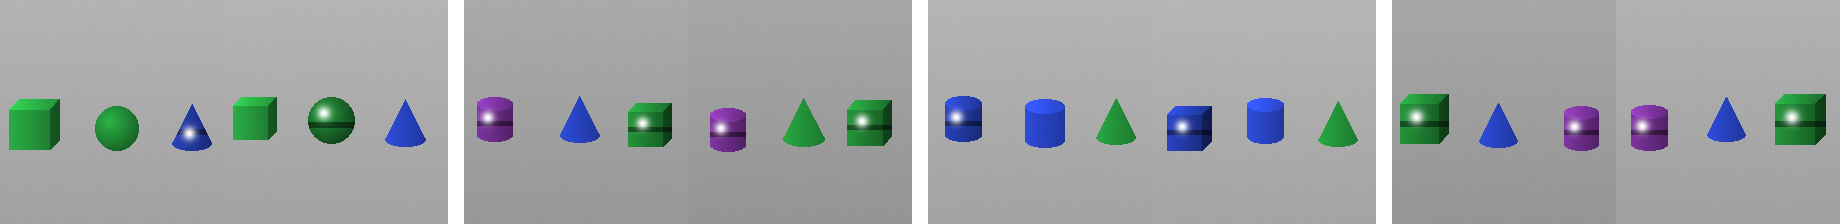
\includegraphics[width=\linewidth]{figures/dev_examples_row.png}
\caption{The first four development groups in generation order (not selected by model
performance). Each pair shows the two members of one group. The pixels are those of the run output
\texttt{dev\_examples.png}, re-tiled into one row by \texttt{scripts/make\_paper\_figures.py}.}
\label{fig:examples}
\end{figure}

\paragraph{Edit orbits and splits.}
Binding and relation edits generate a group action on scenes: transpositions of colours, of
materials or of slots between objects generate all permutations of each attribute type, with shapes
attached to object identities. Ignoring the validity constraint on intermediate scenes, the
\emph{edit orbit} of a scene under this action is the set of valid scenes with the same multisets
of shapes, colours and materials (positions always fill the three slots), and the split key is
exactly this triple of multisets. Attribute and object edits change these multisets and so move a scene to a
different orbit. Data v0 prevented leakage at the level of scenes and caption contents, so all
render variants and paraphrases of a scene or caption stayed in one split. Data v1 adds the orbit
as a leakage unit: every orbit is assigned to one split by a hash of its key, base scenes are drawn
only from the split's orbits, and an edit is kept only if its result stays in an orbit owned by the
same split. This restriction changes the distribution of accepted content edits relative to
unrestricted sampling; Appendix~\ref{app:splits} reports the measured proposal and acceptance
counts instead of assuming uniformity. Data v1 uses a fresh seed and the v0 split sizes
(\DVnTrain{} training, \DVnDev{} development, \DVnCalib{} calibration and \DVnTestIid{},
\DVnTestHeldoutPairs{}, \DVnTestComposition{} and \DVnTestHeldoutTemplate{} groups in the four test
splits). The v0 test splits were scored during an early technical smoke run and are treated as
development material; no model has been scored on any v1 test split.

\paragraph{Binding-necessary endpoint.}
A group is \emph{binding-necessary} (\bn) when all of its edits are binding or relation edits.
Equivalently, both of its scenes lie in the same orbit, so the two images contain the same objects
and attribute values and differ only in their assignment or arrangement. The subset is defined by
metadata alone and never by model scores. It is the primary endpoint because on groups with content
edits a binding-blind signal can succeed: in the v0 smoke run (oracle tokens, first 100 groups of
the v0 composition split), the content-only channel of each trained head reached GroupMatch
\SMcontentMatchMin--\SMcontentMatchMax{}, against a chance level of $0.5$.

\paragraph{Head and scorer.}
The trainable head is shared by all conditions. For a set of image tokens $\{v_k\}_{k=1}^{n}$ it
outputs a content part $c = W_c\,\tfrac1n\sum_k v_k$ and a binding part
$b = \tfrac1n\sum_k (A v_k)\odot(A' v_k)$. For text tokens $\{u_t\}_{t=1}^{L}$ the binding part is
$\tfrac1L\sum_t\sum_{\delta\in\pm\{1..5\}}\alpha_\delta (B u_t)\odot(B' u_{t+\delta})$ with learned
offset weights $\alpha_\delta$. The score is the inner product
$s(I,T)=\langle [c_I;b_I],[c_T;b_T]\rangle$. With 8 content and 8 binding dimensions and
512-dimensional inputs, the head has \SPheadParams{} parameters; the frozen encoder has
\SPencParams. Tokens are standardized per dimension with statistics of the training panel.
With the additive oracle tokens of v0, the content part is exactly invariant to binding and relation
edits by construction. With CLIP tokens this invariance no longer holds, and we measure it instead
of assuming it (Section~\ref{sec:experiments}).

\paragraph{Metrics, ties and chance levels.}
For a group with score matrix $S_{ij}=s(I_i,T_j)$, the Winoground \emph{text} score requires
$S_{00}>S_{01}$ and $S_{11}>S_{10}$, the \emph{image} score requires $S_{00}>S_{10}$ and
$S_{11}>S_{01}$, and the \emph{group} score requires both \citep{thrush2022winoground}.
\emph{GroupMatch} requires $S_{00}+S_{11}>S_{01}+S_{10}$ \citep{zhu2025ttm}. With a meaning-preserving
paraphrase $T'_i$ of each caption, \emph{aug} counts images for which both $T_i$ and $T'_i$ beat
$T_{1-i}$, and \emph{aug\_group} requires this for both images \citep[after][]{kamath2024hardpositive}.
The \emph{pair AUC} treats the four image--caption pairs of each group as a binary ranking problem
labelled by the oracle. All comparisons are strict with a relative tolerance of $10^{-9}$, so ties,
including round-off differences between mathematically equal scores, count as failures. AUC
assigns tied scores their average rank. For independent continuous scores the chance levels are
$1/4$ (text, image), $1/6$ (group), $1/2$ (GroupMatch), $1/3$ (aug), $1/9$ (aug\_group) and $0.5$
(pair AUC). Each is derived separately in Appendix~\ref{app:chance}; we do not transfer the $1/k!$
formula for GroupMatch to other metrics. A Monte-Carlo check on the development panel gives
\SPchanceGroupMC{} for group and \SPchanceMatchMC{} for GroupMatch.

\paragraph{Controls.}
We report an oracle scorer (metadata truth, an upper bound for the evaluation code), zero-shot CLIP
cosine scores, a text-only n-gram logistic regression and an image-only logistic regression on
pooled CLIP features, the content-only and binding-only channels of the trained head, the trained
head with development images or captions shuffled across groups, and the same head trained on
oracle object tokens. On $2{\times}2$ groups a single-modality scorer produces two identical rows or
columns. Every comparison therefore ties, and its text, image, group and GroupMatch scores are zero
by construction. Its pair AUC is exactly $0.5$ because every caption, and every image, appears once
with each label (Appendix~\ref{app:blind}). These values are properties of the design, not evidence
that the benchmark is free of artefacts. For artefacts, the informative checks are the content-only
channel, the shuffles, and classifiers that try to tell base from edited scenes.

\section{Objectives under Study}
\label{sec:method}

\paragraph{Hard-negative contrastive loss.}
A batch contains $B$ groups, hence $2B$ images and $2B$ captions. With $S$ the $2B{\times}2B$
score matrix, the loss $\mathcal{L}_{\mathrm{hn}}$ is the average of row-wise (image$\to$caption)
and column-wise (caption$\to$image) cross-entropies with diagonal targets. Every off-diagonal pair
that the oracle marks as true is removed from the denominators, so it is never used as a negative.
The group partner of each item is kept as a negative (the hard negative). This is the NegCLIP-style
use of minimal-change partners \citep{yuksekgonul2023bow,awal2024vismin}, applied here to a small
head on frozen features.

\begin{remark}[a standard bilinear identity]
\label{rem:identity}
Assume the score is an inner product $s(I,T)=\langle \phi(I),\psi(T)\rangle$, where $\phi$ depends
only on the image and $\psi$ only on the caption. Per-input normalization, as in cosine scores, is
allowed; normalization or attention that depends on the pair is not. Then, for a $2{\times}2$
group,
\begin{equation}
\begin{aligned}
S_{00}+S_{11}-S_{01}-S_{10}
&=\langle\phi(I_0),\psi(T_0)\rangle+\langle\phi(I_1),\psi(T_1)\rangle
-\langle\phi(I_0),\psi(T_1)\rangle-\langle\phi(I_1),\psi(T_0)\rangle\\
&=\langle \phi(I_0)-\phi(I_1),\,\psi(T_0)-\psi(T_1)\rangle ,
\end{aligned}
\label{eq:identity}
\end{equation}
by bilinearity alone. Both the head of Section~\ref{sec:setting} and zero-shot cosine CLIP satisfy
the assumption.
\end{remark}

Equation~\eqref{eq:identity} is elementary; we state it because it fixes what several signals
share. GroupMatch is exactly the event that the right-hand side is positive. The two within-group
row margins of the hard-negative loss, $S_{00}-S_{01}$ and $S_{11}-S_{10}$, sum to the same
quantity. Aligning the image edit vector $\phi(I_1)-\phi(I_0)$ with the caption edit vector
$\psi(T_1)-\psi(T_0)$ of the same group rewards the same inner product, up to normalization. None
of this holds automatically for scorers with pair-dependent computation, such as cross-attention
heads, and we do not apply it to them.

\paragraph{The edit-consistency objective under study.}
For each group $g$ in a batch let $\Delta^I_g=e(I^g_1)-e(I^g_0)$ and $\Delta^T_g=e(T^g_1)-e(T^g_0)$,
using the same member order in both modalities, where $e$ is the concatenated head output. The
objective $\mathcal{L}_{\mathrm{edit}}$ is a symmetric cross-entropy over the $B{\times}B$ matrix
$C_{gh}=\cos(\Delta^I_g,\Delta^T_h)/\tau$ with diagonal targets and $\tau=0.1$. Norms include a
small $\epsilon$, so zero edit vectors give uniform logits and a loss of $\log B$: unlike a squared
error between edit vectors, zero is not a minimizer. The diagonal entries reward the normalized
within-group quantity of Remark~\ref{rem:identity} and therefore overlap with the hard-negative
loss. The off-diagonal entries are the additional signal: an image edit must be closer in direction
to its own caption edit than to the caption edits of other groups in the batch. The objective
assumes that different groups in a batch carry different edits; edit-level false negatives are not
masked. The combined loss is $\mathcal{L}_{\mathrm{hn}}+\lambda\,\mathcal{L}_{\mathrm{edit}}$.

\paragraph{Scale.}
On the first training batch of the small panel, before training and with $\lambda=1$, the ratio
$\|\nabla\mathcal{L}_{\mathrm{edit}}\|/\|\nabla\mathcal{L}_{\mathrm{hn}}\|$ was \SPgradInitMin--\SPgradInitMax{}
across seeds; after hard-negative training it was \SPgradEndMin--\SPgradEndMax. We report these
ratios only to show that $\lambda$ must be small for the two terms to be on comparable scales. A
large gradient says nothing about usefulness.

\section{Experiments and Observations}
\label{sec:experiments}

All numbers are produced by one exporter from the raw run files and inserted as macros
(Appendix~\ref{app:provenance}). Every experiment uses data v1, frozen features, one CPU thread and
development data only. Seeds are optimization repeats on the same panel, not independent samples.

\subsection{Renderer and data audits}
Before any model was run, an audit-only pixel decoder recovered slot, shape, colour and material of
every object from the rendered images. It flagged a renderer error: the specular highlight of metal
cones fell outside the cone's narrow top, so those cones looked like rubber. After the fix, the
decoder found \SPrenderMismatch{} mismatches on all \SPrenderImages{} images of the small panel.
The decoder is a hand-written check written with the renderer, so it shows self-consistency, not
independent visual verification. Data v1 passed all structural and leakage audits (\DVauditFail{}
failures). Logistic-regression detectors that try to tell the base from the edited member reached
AUC \DVblindText{} (caption n-grams) and \DVblindImage{} (oracle tokens) on \DVblindN{}
development and calibration items. A detector on pooled CLIP image features reached
\SPdetectAUC{} with a 95\% bootstrap interval of [\SPdetectLo, \SPdetectHi] on the \SPdetectN{} panel images.
That interval is wide, and none of these linear detectors rules out nonlinear traces.

\subsection{Small development panel: hard-negative baseline}
The baseline was trained with a single setting fixed before the run: learning rate \SPlr, weight
decay \SPwd, \SPsteps{} steps of \SPbatch{} groups, logit scale 1, and seeds 0, 1 and 2. It used the first
\SPtrainGroups{} training and first \SPdevGroups{} development groups of data v1. Half of the
development groups (\SPdevBNn) are binding-necessary. Table~\ref{tab:small} reports the results.

\begin{table}[t]
\caption{Small development panel (\SPtrainGroups{} training / \SPdevGroups{} development groups,
\SPdevBNn{} binding-necessary). Entries for trained heads list seeds 0/1/2, which are optimization
repeats on the same panel. \bn: binding-necessary subset; ``all'': all four edit kinds. Chance for
independent continuous scores: group $1/6$, GroupMatch $1/2$, pair AUC $0.5$. Single-modality rows
are zero or $0.5$ by construction (Section~\ref{sec:setting}). Source:
\url{runs/pixel_baseline_v1_20260926T161957Z/metrics.json}.}
\label{tab:small}
\centering\footnotesize
% GENERATED by scripts/export_paper_numbers.py from runs/pixel_baseline_v1_20260926T161957Z; do not edit by hand.
\begin{tabular}{lcccc}
\toprule
Scorer & \bn{} group & \bn{} GroupMatch & \bn{} pair AUC & all: group \\
\midrule
Oracle (metadata) & 1.00 & 1.00 & 1.00 & 1.00 \\
Zero-shot CLIP & .000 & .688 & .497 & .312 \\
Text-only (n-gram LR) & .000 & .000 & .500 & .000 \\
Image-only (CLIP LR) & .000 & .000 & .500 & .000 \\
\midrule
Pixel head (hard-neg.) & .062/.000/.000 & .625/.500/.438 & .508/.500/.508 & .375/.156/.188 \\
\quad content channel & .000/.000/.000 & .562/.562/.438 & .506/.504/.494 & .219/.156/.188 \\
\quad binding channel & .125/.062/.000 & .625/.625/.562 & .515/.537/.511 & .062/.062/.000 \\
\quad images shuffled & .000/.000/.000 & .312/.312/.375 & .488/.496/.488 & .000/.062/.031 \\
\quad captions shuffled & .000/.000/.000 & .375/.500/.750 & .502/.487/.494 & .062/.000/.000 \\
\quad train-panel fit & .750/.562/.875 & 1.00/1.00/1.00 & .716/.621/.657 & .844/.781/.938 \\
\midrule
Oracle object tokens & .312/.125/.188 & .812/.750/.750 & .619/.548/.569 & .312/.094/.188 \\
\bottomrule
\end{tabular}

\end{table}

\paragraph{Observations.}
(1) The evaluation path behaves as intended. The oracle scores \SPoracleBNGroup, and shuffling
development images or captions across groups drives the \bn{} group score to
\SPimgShufBNGroupMax{} and \SPtxtShufBNGroupMax{} respectively in every seed.
(2) The head largely fits its training groups: on the \SPfitN{}-group fit subset its group score
was \SPfitGroup, and on the full training panel its \bn{} group score was
\SPtrainBNGroupMin--\SPtrainBNGroupMax. The fit is surface-bound, however: on the fit subset,
the aug\_group score with meaning-preserving paraphrases was only \SPfitAugGroup.
(3) On binding-necessary development groups the head is at or below chance: its group score is
\SPdevBNGroupMin--\SPdevBNGroupMax{}, its GroupMatch \SPdevBNMatchMin--\SPdevBNMatchMax{} and
its pair AUC \SPdevBNAUCMin--\SPdevBNAUCMax.
(4) Most of the head's full-panel group score (\SPdevAllGroupMin--\SPdevAllGroupMax) is
reproduced by its content channel alone (\SPcontentAllGroupMin--\SPcontentAllGroupMax).
Zero-shot CLIP shows the same pattern: \SPzsAllGroup{} on all kinds but \SPzsBNGroup{} on the \bn{}
subset, although its \bn{} GroupMatch is \SPzsBNMatch.
(5) The oracle object-token control, whose input already binds attributes, reaches \bn{}
development group scores of only \SPotcBNGroupMin--\SPotcBNGroupMax{} after fitting its training
groups perfectly (\SPotcTrainBNGroupMin). With \SPtrainGroups{} training groups, therefore, the
head and the data size already limit generalization, before any limit of the encoder comes into
play. We cannot separate these factors on this panel, and with \SPdevBNn{} \bn{} groups we make no
significance claim in either direction.

\subsection{Encoder sensitivity diagnostics}
For each development group we compared the cosine distance between the pooled CLIP embeddings of
the two members with the distance between two renders of the same member under different seeds. The
median ratio was \SPnuisObject{} for object edits, \SPnuisAttribute{} for attribute edits,
\SPnuisBinding{} for binding edits and \SPnuisRelation{} for relation edits. Relation swaps
therefore move the pooled embedding about as much as rendering nuisance does. The content channel
is no longer invariant: for binding-necessary pairs rendered with a shared seed, the median relative
content change $\|c(I_1)-c(I_0)\|/\|c(I_0)\|$ was \SPcontentResidMin--\SPcontentResidMax{} across
seeds, whereas with v0 oracle tokens it was zero by construction. The invariance of v0 was a
property of its additive inputs, not something the head learned.

\ifhavepaired
\subsection{Paired comparison with the edit-consistency objective}
\label{sec:paired}

\paragraph{Design, fixed before the run.}
The panel contains the first \SSpanelTrainN{} training groups (\SSpanelTrainOrbits{} orbits) and
\SSpanelDevN{} development groups (\SSpanelDevOrbits{} orbits). The development groups start after
the \SSpanelDevExcluded{} groups already scored in the small-panel stage. The two panels share
\SSpanelOverlap{} orbits, and \PRdevBNN{} of the development groups are binding-necessary. Arm A
uses the hard-negative loss. Arm B adds $\lambda\,\mathcal{L}_{\mathrm{edit}}$ with
$\lambda=\PRlambda$, the smallest non-zero value of the earlier pre-registered grid. We disclose
that this grid was set after observing gradient scales, and $\lambda$ was not changed after any
development result was seen. Both arms share initialization, batch order, supervision,
false-negative masks, cached encoder features, optimizer (AdamW, learning rate \PRlr, weight decay
\PRwd) and \PRsteps{} updates of \PRbatch{} groups. Seeds 0, 1 and 2 are paired optimization
repeats, and the development panel is scored only after the final update. At initialization the
edit gradient was \PRgradInitMean{} times the task gradient (mean over the three first batches), so
$\lambda$ scales it to about \PRgradInitLamMean{} of the task gradient. Encoding the
\PRrenderImages{} panel images and their captions took \PRencCPU{} CPU seconds, and the audit
decoder found \PRrenderMismatch{} mismatches.

\begin{table}[t]
\caption{Paired comparison on \SSpanelTrainN{} training and \SSpanelDevN{} development groups
(\PRdevBNN{} binding-necessary). Seeds 0/1/2 are paired optimization repeats on the same panel.
Chance for independent scores: group $1/6$, GroupMatch $1/2$, pair AUC $0.5$. Source:
\url{runs/paired_v1_20260926T230018Z/paired_summary.json}.}
\label{tab:paired}
\centering\small
% GENERATED by scripts/export_paper_numbers.py from runs/paired_v1_20260926T230018Z; do not edit by hand.
\begin{tabular}{lccc}
\toprule
Seeds 0/1/2 & A: hard-neg. & B: + edit-cons. & B$-$A \\
\midrule
Dev \bn{} group score & .094/.016/.000 & .000/.125/.234 & $-$.094/.109/.234 \\
Dev \bn{} GroupMatch & .688/.641/.656 & .609/.812/.719 & $-$.078/.172/.062 \\
Dev \bn{} pair AUC & .520/.503/.501 & .506/.549/.574 & $-$.014/.045/.073 \\
Dev binding-only group & .156/.000/.000 & .000/.156/.469 & $-$.156/.156/.469 \\
Dev relation-only group & .031/.031/.000 & .000/.094/.000 & $-$.031/.062/.000 \\
Dev all-kinds group & .367/.289/.250 & .297/.383/.461 & $-$.070/.094/.211 \\
Dev all-kinds GroupMatch & .844/.820/.828 & .805/.906/.859 & $-$.039/.086/.031 \\
Train \bn{} group (fit) & .535/.152/.066 & .094/.746/.703 & $-$.441/.594/.637 \\
Final task loss & 0.51/1.83/7.18 & 0.91/0.25/0.29 & 0.40/$-$1.58/$-$6.89 \\
\bottomrule
\end{tabular}

\end{table}

\paragraph{Outcome under the pre-fixed rules.}
Neither arm met the fit criterion, a seed-mean binding-necessary training group score of at least
$0.75$: A reached \PRATrainBNGroupMean{} and B \PRBTrainBNGroupMean{} (Table~\ref{tab:paired}). The
pre-registered verdict is therefore \texttt{\PRverdict}. Training was unstable in both arms. The
task loss oscillated during training, and the largest logged gradient norm per run ranged from
\PRgradMinOfMax{} to \PRgradMaxAll. Arm A finished seed 2 at a task loss of \PRALossLastSeedTwo{},
above its initial value, and seed 1 at \PRALossLastSeedOne. Arm B finished at
\PRBLossLastSeedZero, \PRBLossLastSeedOne{} and \PRBLossLastSeedTwo.

\paragraph{What the difference does and does not show.}
On binding-necessary development groups, the edit-consistency arm scored higher in \PRdiffGroupPos{}
of 3 seeds. The mean paired difference in group score is \PRdiffGroup. Its group-level bootstrap
interval is [\PRdiffGroupLo, \PRdiffGroupHi], but that interval treats the three runs as fixed and
does not reflect their optimization variance. The per-seed differences in Table~\ref{tab:paired} are
positive in the seeds where the baseline ended with a high final loss, and negative in the seed
where it did not. We therefore do not read them as added utility of the objective. Both arms also
sit below the independent-score chance level on the group score (A: \PRACIGroupMean{},
[\PRACIGroupLo, \PRACIGroupHi]; B: \PRBCIGroupMean{}, [\PRBCIGroupLo, \PRBCIGroupHi]) and above it
on GroupMatch (A: \PRACIMatchMean; B: \PRBCIMatchMean). A scorer whose preferences are correlated
across the two captions, for instance one that prefers the same image for both, can fall below
$1/6$ on the group score while still matching better than $1/2$, so the two metrics must be read
together. Zero-shot CLIP on the same subset reaches \PRzsBNGroup{} (group) and \PRzsBNMatch{}
(GroupMatch). Following the pre-fixed rules, the edit-objective branch is put on hold. No
stabilization, encoder change, data increase or new loss was started on the basis of this result.

\else
\subsection{Paired comparison with the edit-consistency objective}
This draft does not yet contain the paired comparison between the hard-negative loss and the same
loss plus the edit-consistency objective. Its fixed design is described in
Appendix~\ref{app:planned}.
\fi

\section{Discussion and Limitations}
\label{sec:discussion}

\paragraph{What the observations support.}
The setting does what it was built to do: model inputs are produced from pixels and caption strings
alone, the evaluation path passes its oracle and shuffle checks, and the binding-necessary subset
removes the part of the metric that a binding-blind channel can solve. On this subset, a
hard-negative head on frozen CLIP tokens fits its training groups on a small panel but does not
transfer to held-out orbits. On a larger panel, under a single fixed optimizer setting, neither the
baseline nor the edit-consistency variant fitted its training groups, and training was unstable. This is a statement about one encoder, one head, one
training setting and small panels. It is neither a claim that the encoder lacks binding
information nor a claim that hard negatives fail in general.

\paragraph{Limitations.}
\emph{Optimization.} The paired comparison used one fixed learning rate, no learning-rate
schedule, no gradient clipping and unnormalized inner-product scores, and it was evaluated only at
the final update. Its per-seed differences are confounded with loss spikes, and its group-level
bootstrap interval ignores run-to-run variance. \emph{Synthetic renders.} The images are stylized renders of four shapes, five colours and two
materials; nothing here concerns natural images, and we did not test whether CLIP maps the words
``metal'' and ``rubber'' onto our rendering. \emph{Frozen encoder.} Only the head is trained, so no
result speaks to what fine-tuning the encoder would do. Only final-layer tokens of one checkpoint
were used, and other layers or token choices were not examined. \emph{Small panels and dependent
repeats.} The development panels are small, and the three seeds share the same data, so their
spread reflects optimization variance only. Non-significant differences are not evidence of
equivalence. \emph{Self-checked renderer.} Our decoder shows that the renderer is internally
consistent, not that an independent observer would read the scenes the same way.
\emph{Data-generation bias.} Keeping orbits within splits requires restricting content edits to
owned orbits, which changes their distribution. Small splits also differ from training in
attribute composition (Appendix~\ref{app:splits}). \emph{Unopened test.}
No v1 test split has been scored, so no result here is confirmatory. \emph{Prior art.} Each
ingredient of the setting and both objectives have close precedents
(Section~\ref{sec:related}); we have not established novelty for any of them. \emph{Authorship.}
The code and this text were produced by an AI system and have not yet been reviewed by a human
author.

\section{Conclusion}
\label{sec:conclusion}

A binding evaluation is only as informative as the weakest of its inputs, metrics and controls. By
removing oracle features from the model input, splitting at the level of edit orbits and scoring a
metadata-defined binding-necessary subset, we obtained a setting in which a simple hard-negative
head on frozen CLIP tokens can be seen to fit its training groups without transferring to held-out
orbits, and in which blind controls are recognized as structurally uninformative.
\ifhavepaired
The paired comparison with the edit-consistency objective under study did not resolve whether it
adds anything to the hard-negative loss. Neither arm fitted its training groups under the fixed
update budget, both training runs were unstable, and the per-seed differences track which baseline
runs ended with a high final loss. A useful next step would stabilize optimization under a new
pre-registered configuration before comparing objectives again. The v1 test splits remain unopened.

\else
Whether the edit-consistency objective under study adds anything to the hard-negative loss in this
setting is still open. The fixed plan for that comparison is given in Appendix~\ref{app:planned}.
\fi

\label{end-of-main-text}

\subsection*{AI use statement}
This working draft, the code base and every experiment it reports were produced by an AI coding
assistant (Anthropic's Claude, used through Claude Code) acting on a researcher's written
instructions. The assistant designed and implemented the generator, renderer, head, losses and
evaluation code; ran all experiments; verified bibliographic metadata through arXiv's BibTeX export
and paper pages; and wrote this text. AI sub-agents searched and read related work, and their
reports were partially re-checked by the main assistant. \textbf{HUMAN\_REVIEW\_PENDING:} no human
author has yet checked the code, the numbers or the text, and no human is named as having verified
anything. The draft must not be submitted before that review. The repository file
\texttt{AI\_USAGE.md} lists the AI's design decisions and the errors it found and corrected.

\subsection*{Reproducibility statement}
Section~\ref{sec:setting} and Appendices~\ref{app:splits}--\ref{app:planned} describe the data,
splits, inputs, head, objectives and metrics. Every number in the text is generated from raw run
files by \texttt{scripts/export\_paper\_numbers.py}, which writes a provenance table mapping each
macro to a file and field (Appendix~\ref{app:provenance}). Run directories contain configuration,
logs and manifests with code, configuration and data hashes, the environment, wall and CPU time,
and peak memory. The encoder checkpoint is pinned by revision and SHA-256, and Python packages are
pinned in \texttt{requirements-pixel.lock}.


\bibliography{references}
\bibliographystyle{iclr2027_conference}

\appendix
\section{Chance levels of the group metrics}
\label{app:chance}

Let the four scores of a group, $S_{00},S_{01},S_{10},S_{11}$, and the paraphrase scores
$S'_0,S'_1$ be independent draws from one continuous distribution, so ties have probability zero.
These are properties of random scores, not of any trained model. Each metric is derived separately.

\emph{Text and image scores.} The text score needs $S_{00}>S_{01}$ and $S_{11}>S_{10}$. These two
events involve disjoint pairs of independent exchangeable variables, so the probability is
$\tfrac12\cdot\tfrac12=\tfrac14$. The image score is analogous.

\emph{Group score.} All four inequalities hold iff $\min(S_{00},S_{11})>\max(S_{01},S_{10})$, that
is, iff the two diagonal entries are the two largest of four exchangeable values. All
$\binom{4}{2}=6$ pairs are equally likely to be the top two, so the probability is $1/6$.

\emph{GroupMatch.} $X=S_{00}+S_{11}$ and $Y=S_{01}+S_{10}$ are independent and identically
distributed, so $P(X>Y)=1/2$. For $k{\times}k$ groups \citet{zhu2025ttm} give $1/k!$ for GroupMatch
and $(k-1)!/(2k-1)!$ for the group score; we use only $k=2$ and do not carry either formula over to
the other metrics.

\emph{aug.} For image $i$, the other caption must score below both $S_{ii}$ and $S'_i$, that is, be
the smallest of three exchangeable values: probability $1/3$.

\emph{aug\_group.} The two images use the disjoint triples $(S_{00},S'_0,S_{01})$ and
$(S_{11},S'_1,S_{10})$, so the two events are independent and the probability is $1/9$.

\emph{Pair AUC.} Under random scores, the expected AUC is $1/2$.

\section{Splits and metadata statistics}
\label{app:splits}

Orbit ownership is decided by a hash of the orbit key and the data seed, with fractions \DVpartTrain{}
(training), \DVpartDev{} (development), \DVpartCalib{} (calibration), \DVpartTestIid{} for each of the
i.i.d., held-out-pair and composition test splits, and \DVpartTestTemplate{} for the held-out-template
test split (\texttt{configs/data\_v1.json}). For each split, the
generator draws a base scene until its orbit is owned. It then samples an edit of the scheduled kind
among the applicable edits whose result stays in an owned orbit, and it keeps the group only if the
oracle truth table, the operation contract, the held-out-pair rule and the scene/caption-content
registry all pass. Edit kinds follow a fixed cycle, so accepted kinds are balanced within each
split. Content edits (attribute and object edits) are the only edits that can leave an orbit, and
only they are affected by the ownership filter.
\ifhavesplitsemantics
Table~\ref{tab:splits} reports the metadata of every data-v1 split, recomputed by
\texttt{scripts/analyze\_split\_semantics.py} from the generator's own bookkeeping. No model is
involved and no test score is opened. Of the \SSorbitsTotal{} orbits of three-object scenes, each
split owns a hashed subset. ``Content filter keep'' is the fraction of applicable attribute and
object edits whose result stays in an orbit owned by the same split. Binding and relation edits
never leave their orbit, and all of them were kept.

\begin{table}[h]
\caption{Data-v1 split metadata (source:
\url{runs/split_semantics_v1_20260926T230848Z/split_semantics.json}). ``Attempts'' counts every
proposal, including rejected base scenes; ``accept'' is groups divided by attempts; ``orbits'' is
orbits owned, ``used'' orbits occurring in the split; ``keep'' is the content-edit filter keep rate;
\bn{} is the binding-necessary share.}
\label{tab:splits}
\centering\footnotesize
% GENERATED by scripts/export_paper_numbers.py from runs/split_semantics_v1_20260926T230848Z; do not edit by hand.
\begin{tabular}{lrrrrrrr}
\toprule
Split & groups & attempts & accept & orbits & used & keep & \bn{} \\
\midrule
train & 2000 & 6743 & 29.7\% & 1241 & 758 & 50.1\% & 50.0\% \\
dev & 300 & 7063 & 4.2\% & 173 & 97 & 10.4\% & 50.0\% \\
calib & 300 & 19334 & 1.6\% & 176 & 91 & 4.7\% & 50.0\% \\
test i.i.d. & 400 & 6858 & 5.8\% & 241 & 121 & 10.6\% & 50.0\% \\
test held-out pairs & 400 & 14309 & 2.8\% & 243 & 146 & 10.0\% & 50.0\% \\
test composition & 400 & 25297 & 1.6\% & 245 & 149 & 10.9\% & 30.0\% \\
test held-out template & 400 & 80837 & 0.5\% & 121 & 68 & 3.4\% & 50.0\% \\
\bottomrule
\end{tabular}

\end{table}

\paragraph{Consequences.}
(i) Accepted content edits are not a uniform sample of applicable edits. In the development split,
\SSDevReplColorKept{} of \SSDevReplColorAppl{} applicable colour replacements and
\SSDevReplShapeKept{} of \SSDevReplShapeAppl{} applicable shape replacements survived the
ownership filter, while \SSDevSwapColorKept{} of \SSDevSwapColorAppl{} colour swaps did.
Calibration and held-out-template splits keep even fewer content edits (\SSCalibContentFilter{} and
\SSHeldTemplateContentFilter). (ii) Small splits own few orbits, so their attribute composition
differs from training. The total-variation distance to the training colour distribution is
\SSDevTVColor{} for the development split. In the paired development panel green and purple have
frequencies \SSpanelDevColorGreen{} and \SSpanelDevColorPurple{}, against red and blue at
\SSpanelDevColorRed{} and \SSpanelDevColorBlue{}; in the training panel the figures are
\SSpanelTrainColorGreen{}, \SSpanelTrainColorPurple{}, \SSpanelTrainColorRed{} and
\SSpanelTrainColorBlue. (iii) Edit kinds are balanced by construction: half of each single-edit
split is binding-necessary, and \SSpanelDevBN{} of the paired development panel is. (iv) The
analysis was first run on an uncommitted tree and then re-run on the committed code. The two
outputs agree except for one total-variation value that differs in the last floating-point digit
because of summation order. Both runs are kept.

\else
Proposal and acceptance counts per split have not yet been extracted in this draft.
\fi

\section{Structural properties of single-modality scorers}
\label{app:blind}

Let a text-only scorer assign $S_{ij}=f(T_j)$. Then $S_{00}=S_{10}$ and $S_{01}=S_{11}$.
\begin{itemize}
\item The text score needs $f(T_0)>f(T_1)$ and $f(T_1)>f(T_0)$, which is impossible.
\item The image score needs $S_{00}>S_{10}$, a tie.
\item GroupMatch compares $f(T_0)+f(T_1)$ with itself.
\item aug\_group needs the text-score inequalities again.
\end{itemize}
With strict comparisons all four are therefore zero for every $f$. The per-image aug score can
still reach $1/2$, so it is not blind-proof. For the pair AUC, the four pairs of a group carry
labels given by the identity truth table. Each caption $T_j$ appears once with label 1 (with
$I_j$) and once with label 0 (with $I_{1-j}$), with the same score $f(T_j)$. The multisets of
positive and negative scores are therefore identical. The Mann--Whitney statistic, with ties
counted as $1/2$, then equals $1/2$ exactly. The image-only case is symmetric. These identities hold
for any single-modality scorer, including ones that exploit real artefacts, so the corresponding
table entries carry no information about artefacts.

\section{Small-panel results over all edit kinds}
\label{app:full}

\begin{table}[h]
\caption{Small development panel, metrics over all four edit kinds (same run, rows and conventions
as Table~\ref{tab:small}). These include groups that a binding-blind content signal can solve.}
\centering\footnotesize
% GENERATED by scripts/export_paper_numbers.py from runs/pixel_baseline_v1_20260926T161957Z; do not edit by hand.
\begin{tabular}{lccc}
\toprule
Scorer & all: group & all: GroupMatch & all: pair AUC \\
\midrule
Oracle (metadata) & 1.00 & 1.00 & 1.00 \\
Zero-shot CLIP & .312 & .844 & .583 \\
Text-only (n-gram LR) & .000 & .000 & .500 \\
Image-only (CLIP LR) & .000 & .000 & .500 \\
\midrule
Pixel head (hard-neg.) & .375/.156/.188 & .812/.750/.719 & .579/.571/.572 \\
\quad content channel & .219/.156/.188 & .781/.781/.719 & .579/.570/.569 \\
\quad binding channel & .062/.062/.000 & .500/.562/.562 & .507/.514/.513 \\
\quad images shuffled & .000/.062/.031 & .312/.406/.438 & .498/.493/.500 \\
\quad captions shuffled & .062/.000/.000 & .469/.562/.656 & .519/.490/.497 \\
\quad train-panel fit & .844/.781/.938 & 1.00/1.00/1.00 & .758/.725/.745 \\
\midrule
Oracle object tokens & .312/.094/.188 & .906/.781/.875 & .620/.571/.576 \\
\bottomrule
\end{tabular}

\end{table}

\section{Planned experiments (NOT RUN)}
\label{app:planned}

None of the following has been executed; no result in the main text depends on them.
\begin{enumerate}
\ifhavepaired\else
\item \textbf{Paired comparison (planned for this revision).} Two arms, the hard-negative loss (A)
and the same loss plus $\lambda\,\mathcal{L}_{\mathrm{edit}}$ (B). Both use the same
initialization, batches, supervision, false-negative masks, head, cached encoder features,
optimizer and number of updates. $\lambda=0.01$, the smallest non-zero value of the earlier
pre-registered grid; that grid was itself set after gradient-scale observations, which we
disclose. The panel is 512 training and 128 development groups inside the data-v1 training and
development orbits. Seeds 0, 1 and 2 serve as paired optimization repeats. The primary endpoint is
the binding-necessary development group score.
\fi
\ifhavepaired
\item \textbf{Stabilized paired comparison.} The paired comparison of Section~\ref{sec:paired} was
not repeated with a lower learning rate, a schedule, gradient clipping, normalized scores or
checkpoint averaging. Any such change would need a new configuration fixed before running.
\fi
\item \textbf{Test evaluation.} No v1 test split has been rendered, encoded or scored.
\item \textbf{Natural images and encoder fine-tuning.} Not attempted. No natural-image data was
used, and the encoder stays frozen.
\item \textbf{Other encoders, layers or token choices.} Not attempted (single encoder, final layer).
\item \textbf{Calibrated pair accuracy.} Requires a calibration panel, which has not been fixed.
\item \textbf{Edit-loss hyperparameter sweep.} The earlier 12-setting sweep was withdrawn and not
run.
\end{enumerate}

\section{Provenance and corrections}
\label{app:provenance}

\texttt{scripts/export\_paper\_numbers.py} reads the raw run files, writes every number as a macro
to \texttt{paper/generated/numbers.tex}, builds the tables from the same values, and records file,
field and derivation rule per macro in \texttt{paper/generated/provenance.tsv}. Corrections made
during the project are recorded rather than hidden:
\begin{itemize}
\item \emph{Renderer.} The metal-cone highlight error was found by the audit decoder and fixed
before any model was run.
\item \emph{First pixel-stage run.} It was executed on an uncommitted working tree. A re-run at the
committed code gave identical metrics, decisions and parameter hashes, and both runs are kept.
\item \emph{Manifest.} The ``dirty'' flag in the reference run's manifest is a false positive
caused by a parsing bug, since fixed; the recorded source-tree hash identifies the code.
\item \emph{Installation.} A first package-installation attempt failed because a timing utility
was missing; its log is kept.
\end{itemize}


\end{document}
